\documentclass[letterpaper]{article}
\newcounter{qcounter}
\usepackage[nogin]{Sweave}
\usepackage[utf8]{inputenc}
\usepackage{amsmath}
\parskip 7.2pt

\title{Homework 04 Key. PLS206 Fall 2014}
\author{Emilio A. Laca}

\begin{document}
\input{HW04BullsKey-concordance}

\maketitle

{\bf \Large Regression diagnostics and remedial measures}

Use the Bulls.txt data file. The homework consists in checking the assumptions and proposing remedial measures for the regression of SalePr on all the other variables EXCEPT Breed. For this exercise we are using the data as if the goal were to predict bull sale price based on a series of measurable characteristics of animals. Although the goal is prediction, we will be concerned about collinearity because it can inflate the PRESS and reduce the actual precision of predictions for bulls that were not included in the data used to develop the model. Keep in mind that for the application in a "real-world" situation one would not need to predict the sale price for bulls used to develop the model. Sale prices for those bulls are known, albeit with measurement and process error. 

Use the class notes file PLS206Ch08MLR3.docx to guide your work and the pdf file found in http://www.sagepub.com/upm-data/38503_Chapter6.pdf and PLS206Ch04assumpSS.docx to interpret results.
\begin{list}{ \bf \arabic{qcounter}. }{\usecounter{qcounter}}


{\item \bf Do a multiple linear regression of SalePr on YrHgt, FtFrBody, PrctFFB, Frame, BkFat, SaleHt and SaleWt}

Report the minimum output to support your tests. For each test required in each question below, make sure to list remedial measures that can address problems identified. If no remedial measure is required, state so. Do not  apply remedial measures unless you are specifically asked to do it.

\begin{Schunk}
\begin{Sinput}
> bulls <- read.csv("~/Documents/Bulls.txt", header=TRUE)
> names(bulls)
\end{Sinput}
\begin{Soutput}
[1] "Breed"    "SalePr"   "YrHgt"    "FtFrBody" "PrctFFB"  "Frame"    "BkFat"   
[8] "SaleHt"   "SaleWt"  
\end{Soutput}
\begin{Sinput}
> bull1 <- lm(SalePr ~ YrHgt + FtFrBody + PrctFFB + Frame + BkFat
+             + SaleHt + SaleWt, bulls)
> summary(bull1)
\end{Sinput}
\begin{Soutput}
Call:
lm(formula = SalePr ~ YrHgt + FtFrBody + PrctFFB + Frame + BkFat + 
    SaleHt + SaleWt, data = bulls)

Residuals:
    Min      1Q  Median      3Q     Max 
-927.31 -279.95  -43.97  220.15 1612.87 

Coefficients:
              Estimate Std. Error t value Pr(>|t|)   
(Intercept) -3156.8944  4105.7192  -0.769  0.44461   
YrHgt          25.9314   111.4029   0.233  0.81664   
FtFrBody       -2.2012     1.0707  -2.056  0.04365 * 
PrctFFB       -30.0976    26.7168  -1.127  0.26390   
Frame         360.3168   172.9033   2.084  0.04093 * 
BkFat        2571.5500   790.7881   3.252  0.00179 **
SaleHt         84.3969    64.0910   1.317  0.19232   
SaleWt          0.3634     0.6085   0.597  0.55233   
---
Signif. codes:  0 ‘***’ 0.001 ‘**’ 0.01 ‘*’ 0.05 ‘.’ 0.1 ‘ ’ 1

Residual standard error: 460.9 on 68 degrees of freedom
Multiple R-squared:  0.5037,	Adjusted R-squared:  0.4526 
F-statistic: 9.859 on 7 and 68 DF,  p-value: 2.008e-08
\end{Soutput}
\end{Schunk}

{\item \bf Test the assumption of normality. [10]}
\begin{Schunk}
\begin{Sinput}
> library(car)
> shapiro.test(residuals(bull1))
\end{Sinput}
\begin{Soutput}
	Shapiro-Wilk normality test

data:  residuals(bull1)
W = 0.9253, p-value = 0.0002499
\end{Soutput}
\end{Schunk}
\begin{Schunk}
\begin{Sinput}
> qqPlot(bull1, main="QQ Plot") #qq plot for studentized resid
\end{Sinput}
\end{Schunk}
Both the Shapiro-Wilk test and the quantile plot show a significant lack of normality.


\begin{figure}
\begin{center}
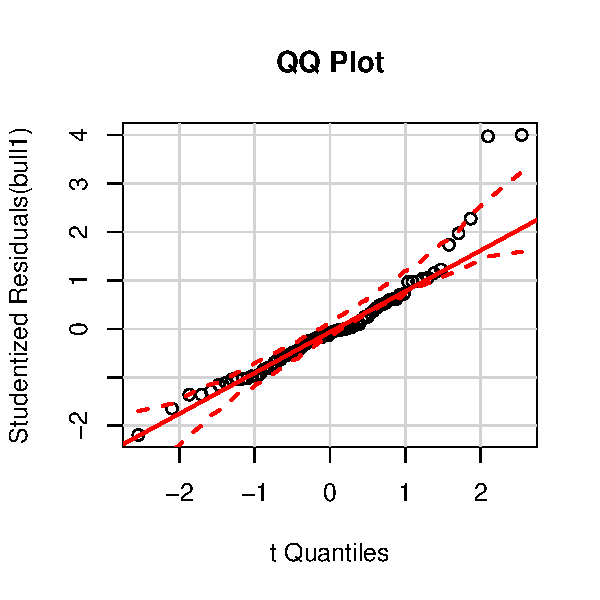
\includegraphics{HW04BullsKey-figqq}
\end{center}
\caption{Quantile plot of residuals to test for normality. There is a significant deviation from normality.}
\label{fig:qq}
\end{figure}

{\item \bf Test the homogeneity of variance. In addition to other potential checks, use Breed as grouping variable. [10]}

\begin{Schunk}
\begin{Soutput}
           Test stat Pr(>|t|)
YrHgt          0.677    0.501
FtFrBody      -0.715    0.477
PrctFFB       -1.565    0.122
Frame          0.528    0.599
BkFat         -1.197    0.235
SaleHt         0.146    0.884
SaleWt        -0.256    0.799
Tukey test     4.441    0.000
\end{Soutput}
\end{Schunk}

\begin{figure}
\begin{center}
\begin{Schunk}
\begin{Soutput}
           Test stat Pr(>|t|)
YrHgt          0.677    0.501
FtFrBody      -0.715    0.477
PrctFFB       -1.565    0.122
Frame          0.528    0.599
BkFat         -1.197    0.235
SaleHt         0.146    0.884
SaleWt        -0.256    0.799
Tukey test     4.441    0.000
\end{Soutput}
\end{Schunk}
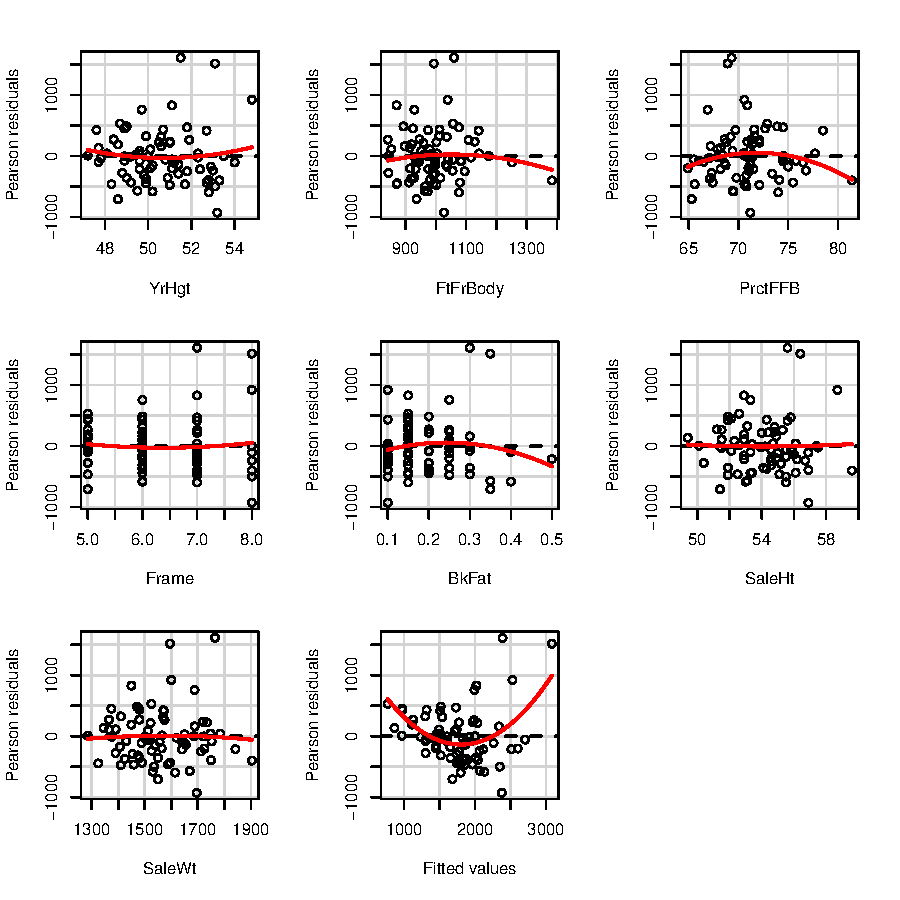
\includegraphics{HW04BullsKey-figHov}
\end{center}
\caption {Residuals are plotted against each predictor and fitted values to assess homogeneity of variance.}
\end{figure}

\begin{Schunk}
\begin{Sinput}
> library(HH)